\chapter{Path Planing In Compositional Spaces through Graph Traversals} \label{chap:pathplanning}

\acknowledge{
This chapter is part of work described in Chapter \ref{chap:infeasibilitygliding} and carries the same acknowledgments.
}

\section{Introduction} \label{pathplan:sec:intro}

Once (1) models developed in Chapters \ref{chap:sipfenn} through \ref{chap:nimcso} are available, and (2) the approach to traversing the compositional space established in Chapters \ref{chap:nimplex} and \ref{chap:infeasibilitygliding} is deployed, one can begin to design multi-composition entities, such as coexisting compositional regions on paths joining multiple compositions in Functionally Graded Alloys (FGMs) discussed in Section~\ref{nimplex:ssec:functionallygraded}. In general, this will entail constructing continuous composition sub-graphs based on certain value rules allowing one to optimize the design.

All results and figures presented throughout this Chapter have been obtained and can be reproduces based on the second \texttt{nimplex} workshop, which has been adapted as Appendix~\ref{chap:nimplextutorial2} and can be consulted for step-by-step details, including an example implementation, which can be easily modified to work in a variety of problems with minimal changes.

\section{Shortest Path Planning} \label{pathplan:sec:shortest}

The most common and most simply defined task in the FGM path planning is to identify a short \cite{Bobbio2022DesignCompositions} or the shortest path. Figure~\ref{pathplan:sec:shortest} presents an example of such path, constructed using Dijkstra's algorithm \cite{Dijkstra1959AGraphs} between two points of choice, over the feasable space graph extracted from results underlying Figure~\ref{infeasibilitygliding:fig:glide} discussed in the last chapter. 

\begin{figure}[H]
    \centering
    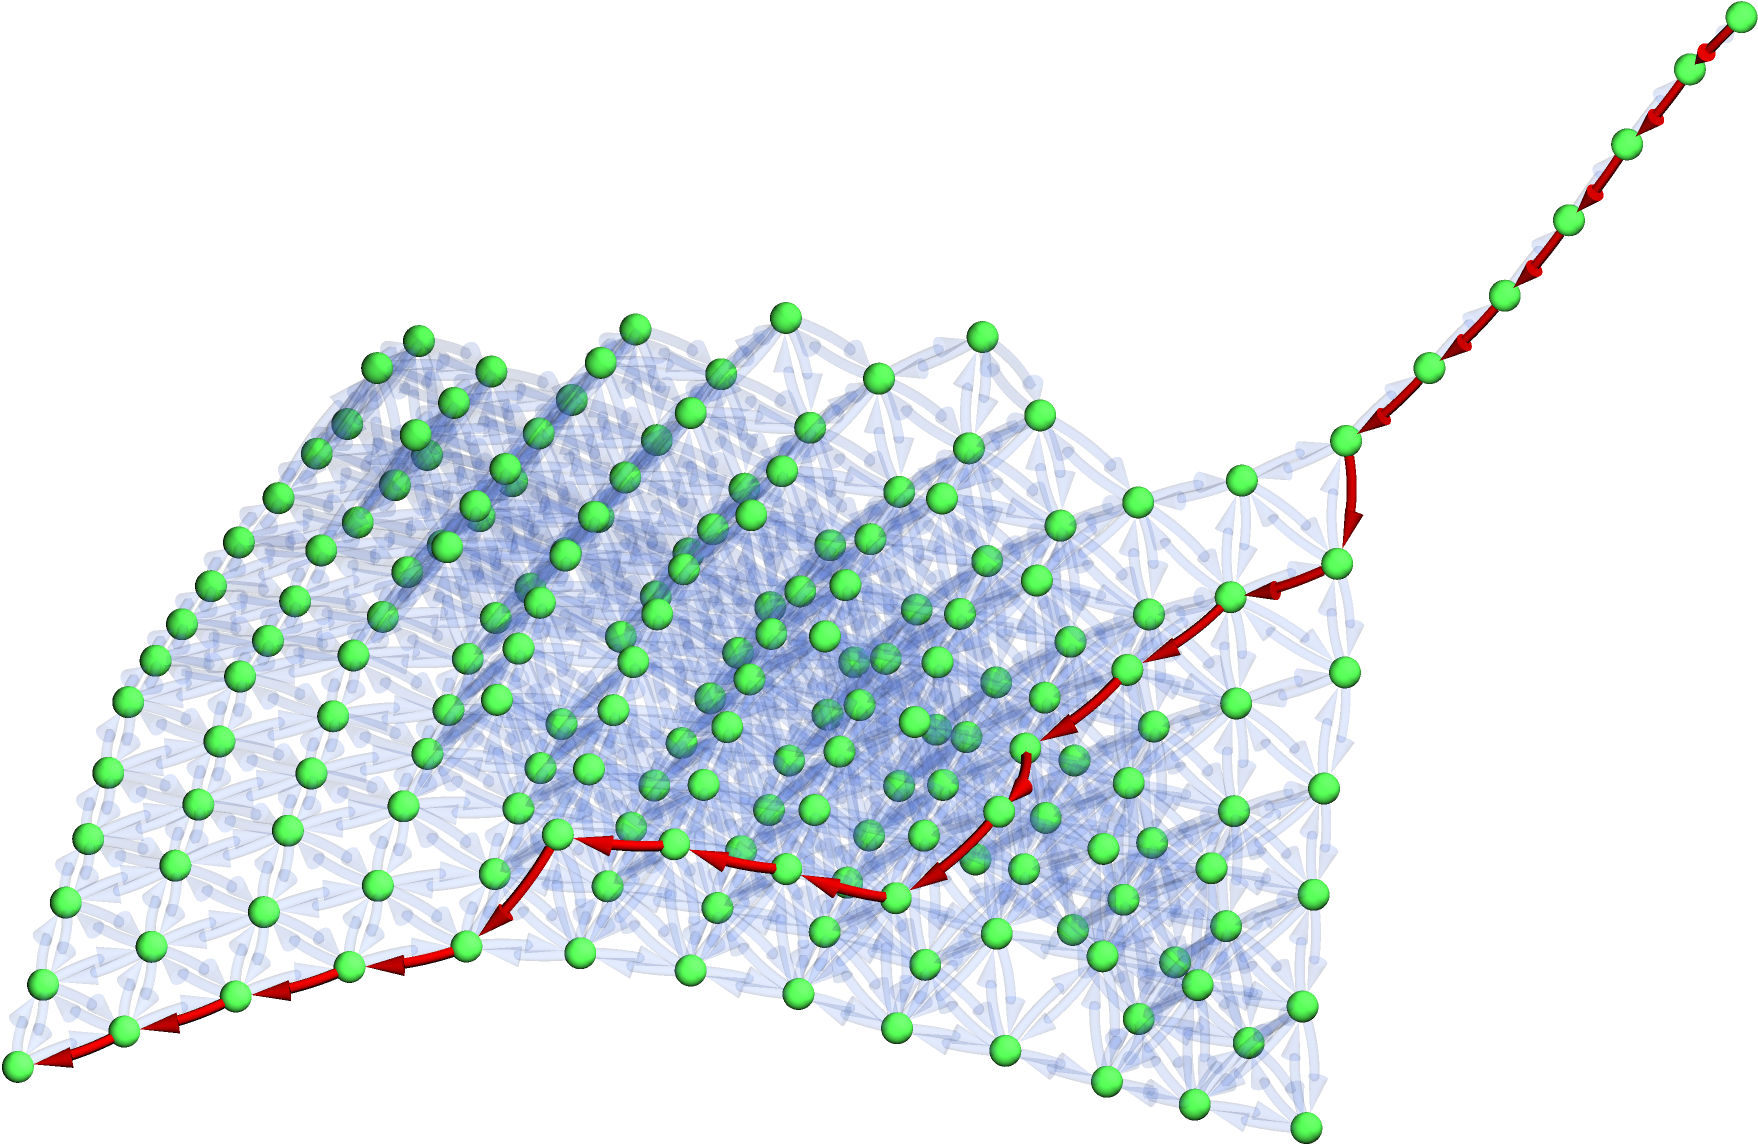
\includegraphics[width=0.9\textwidth]{pathplanning/InfeasibilityGliding_Feasible.png}
    \caption{The subgraph of feasible space extracted from full 3-simplex (tetrahedral) graph in Figure \ref{infeasibilitygliding:fig:glide} constructed by gliding around infeasible region of compositional space. The red path overlaid over directional edges indicates the optimal (least number of transitions) path was identified by the common Dijkstra's algorithm \cite{Dijkstra1959AGraphs}.}
    \label{pathplan:fig:shortestpath}
\end{figure}

Notably, the depicted path belongs to a \emph{set of several equivalent shortest paths} between the two considered points. This situation is similar to more common path plannings on rectangular grids; however, as explored in Chapter~\ref{chap:nimplex}, the number of possible transitions from each point in increasingly dimensional simplex space grows much faster ($d(d-1)$) relative to corresponding Cartesian space ($2d$), what can have a significant effect on memory requirements of certain planning algorithms.

\section{Property Gradient Minimization} \label{pathplan:sec:gradientmin}

As demonstrated in detail in Appendix~\ref{chap:nimplextutorial2}, \texttt{nimplex} graph representations offer a very flexible framework for encoding additional characteristics of the problem at hand, like the common FGM-related task of minimization of thermal expansion coefficient (TCE) gradients \cite{Kirk2021ComputationalMonotonicity} to avoid cracking at elevated temperatures, or elastic modulus gradients to avoid cracking in certain stress conditions.



\subsection{Stretching the Space} \label{pathplan:ssec:gradientstretch}

One can, for instance, stretch the edges between points shown earlier in the Figure~\ref{pathplan:fig:shortestpath} by adding a penalty linearly proportional to the magnitude of the gradient of a property value. In the Appendix~\ref{chap:nimplextutorial2}, an exmaple property of choice has been the Root Mean Square Average Deviation (RMSAD) model for BCC solid solutions by \citet{Tandoc2023MiningAlloys}, modified to fit ULTERA model pattern. The result of such stretching is shown in Figure~\ref{pathplan:fig:lowgradient}, where the path has been biased towards low-gradient regions achieving the singular shortest design path under such conditions. 

\begin{figure}[H]
    \centering
    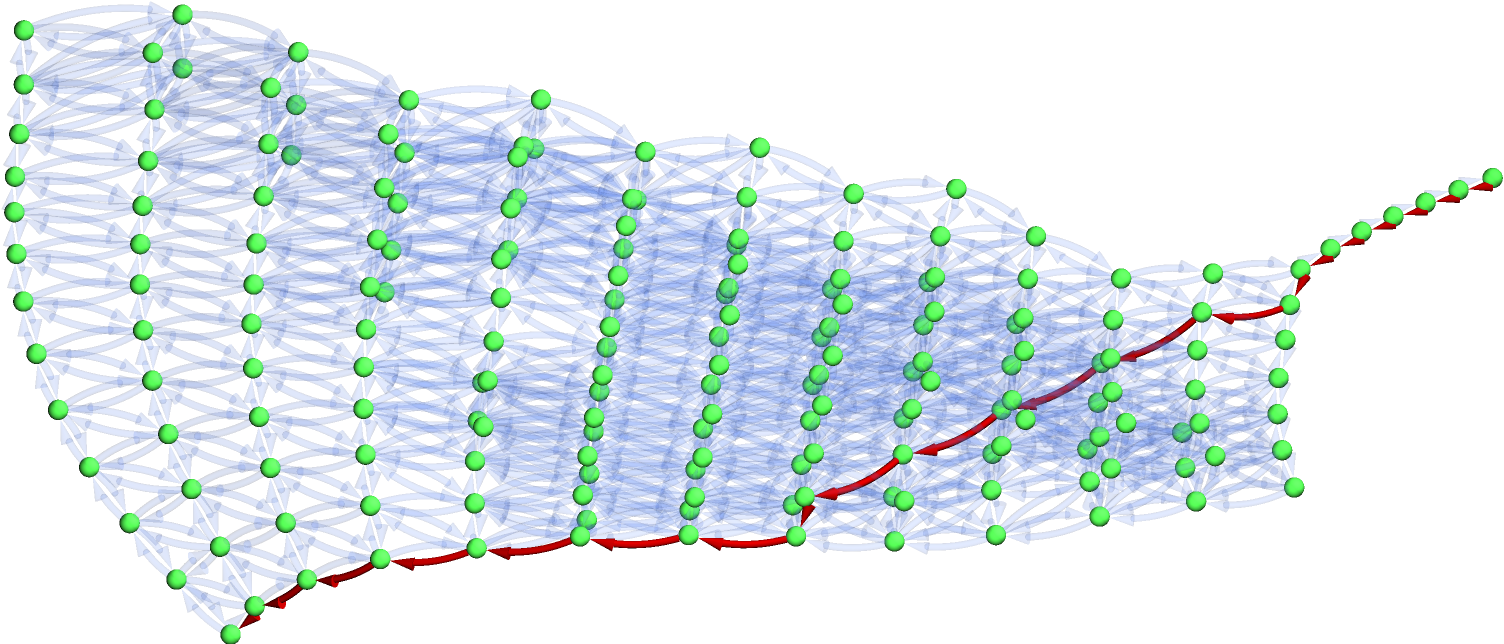
\includegraphics[width=0.9\textwidth]{pathplanning/InfeasibilityGliding_LowGradient.png}
    \caption{The graph from Figure \ref{pathplan:fig:shortestpath} stretched through distance increases from penalizing high magnitude of gradient in a property value. The graph is approximately relaxed through spring-type energy minimization performed in Wolfram Language. The shortest path is still equally optimal in terms of number of steps but the selection has been biased towards low-gradient region.}
    \label{pathplan:fig:lowgradient}
\end{figure}

Notably, while the resulting path is different compared to one in Figure~\ref{pathplan:fig:shortestpath}, it still belongs to the set of shortest paths in terms of unstretched distance (number of transitions) for any scale of gradient penalty, as neighboring derivative paths are similarily affected by the penalty.

\subsection{Non-Linear Penalties Escaping Embedding} \label{pathplan:ssec:gradientsquare}

Introduction of a non-linear gradient results in distances cannot be easily visualized as stretching of the space, as depicted in Figure~\ref{pathplan:fig:lowgradientsquared}, but can encode avoidance of singular gradient changes, which can be much more critical in the design of FGMs deposited layer-by-layer where resistance to cracking may be primarily dependent on a few most vounurable tranistions.

\begin{figure}[H]
    \centering
    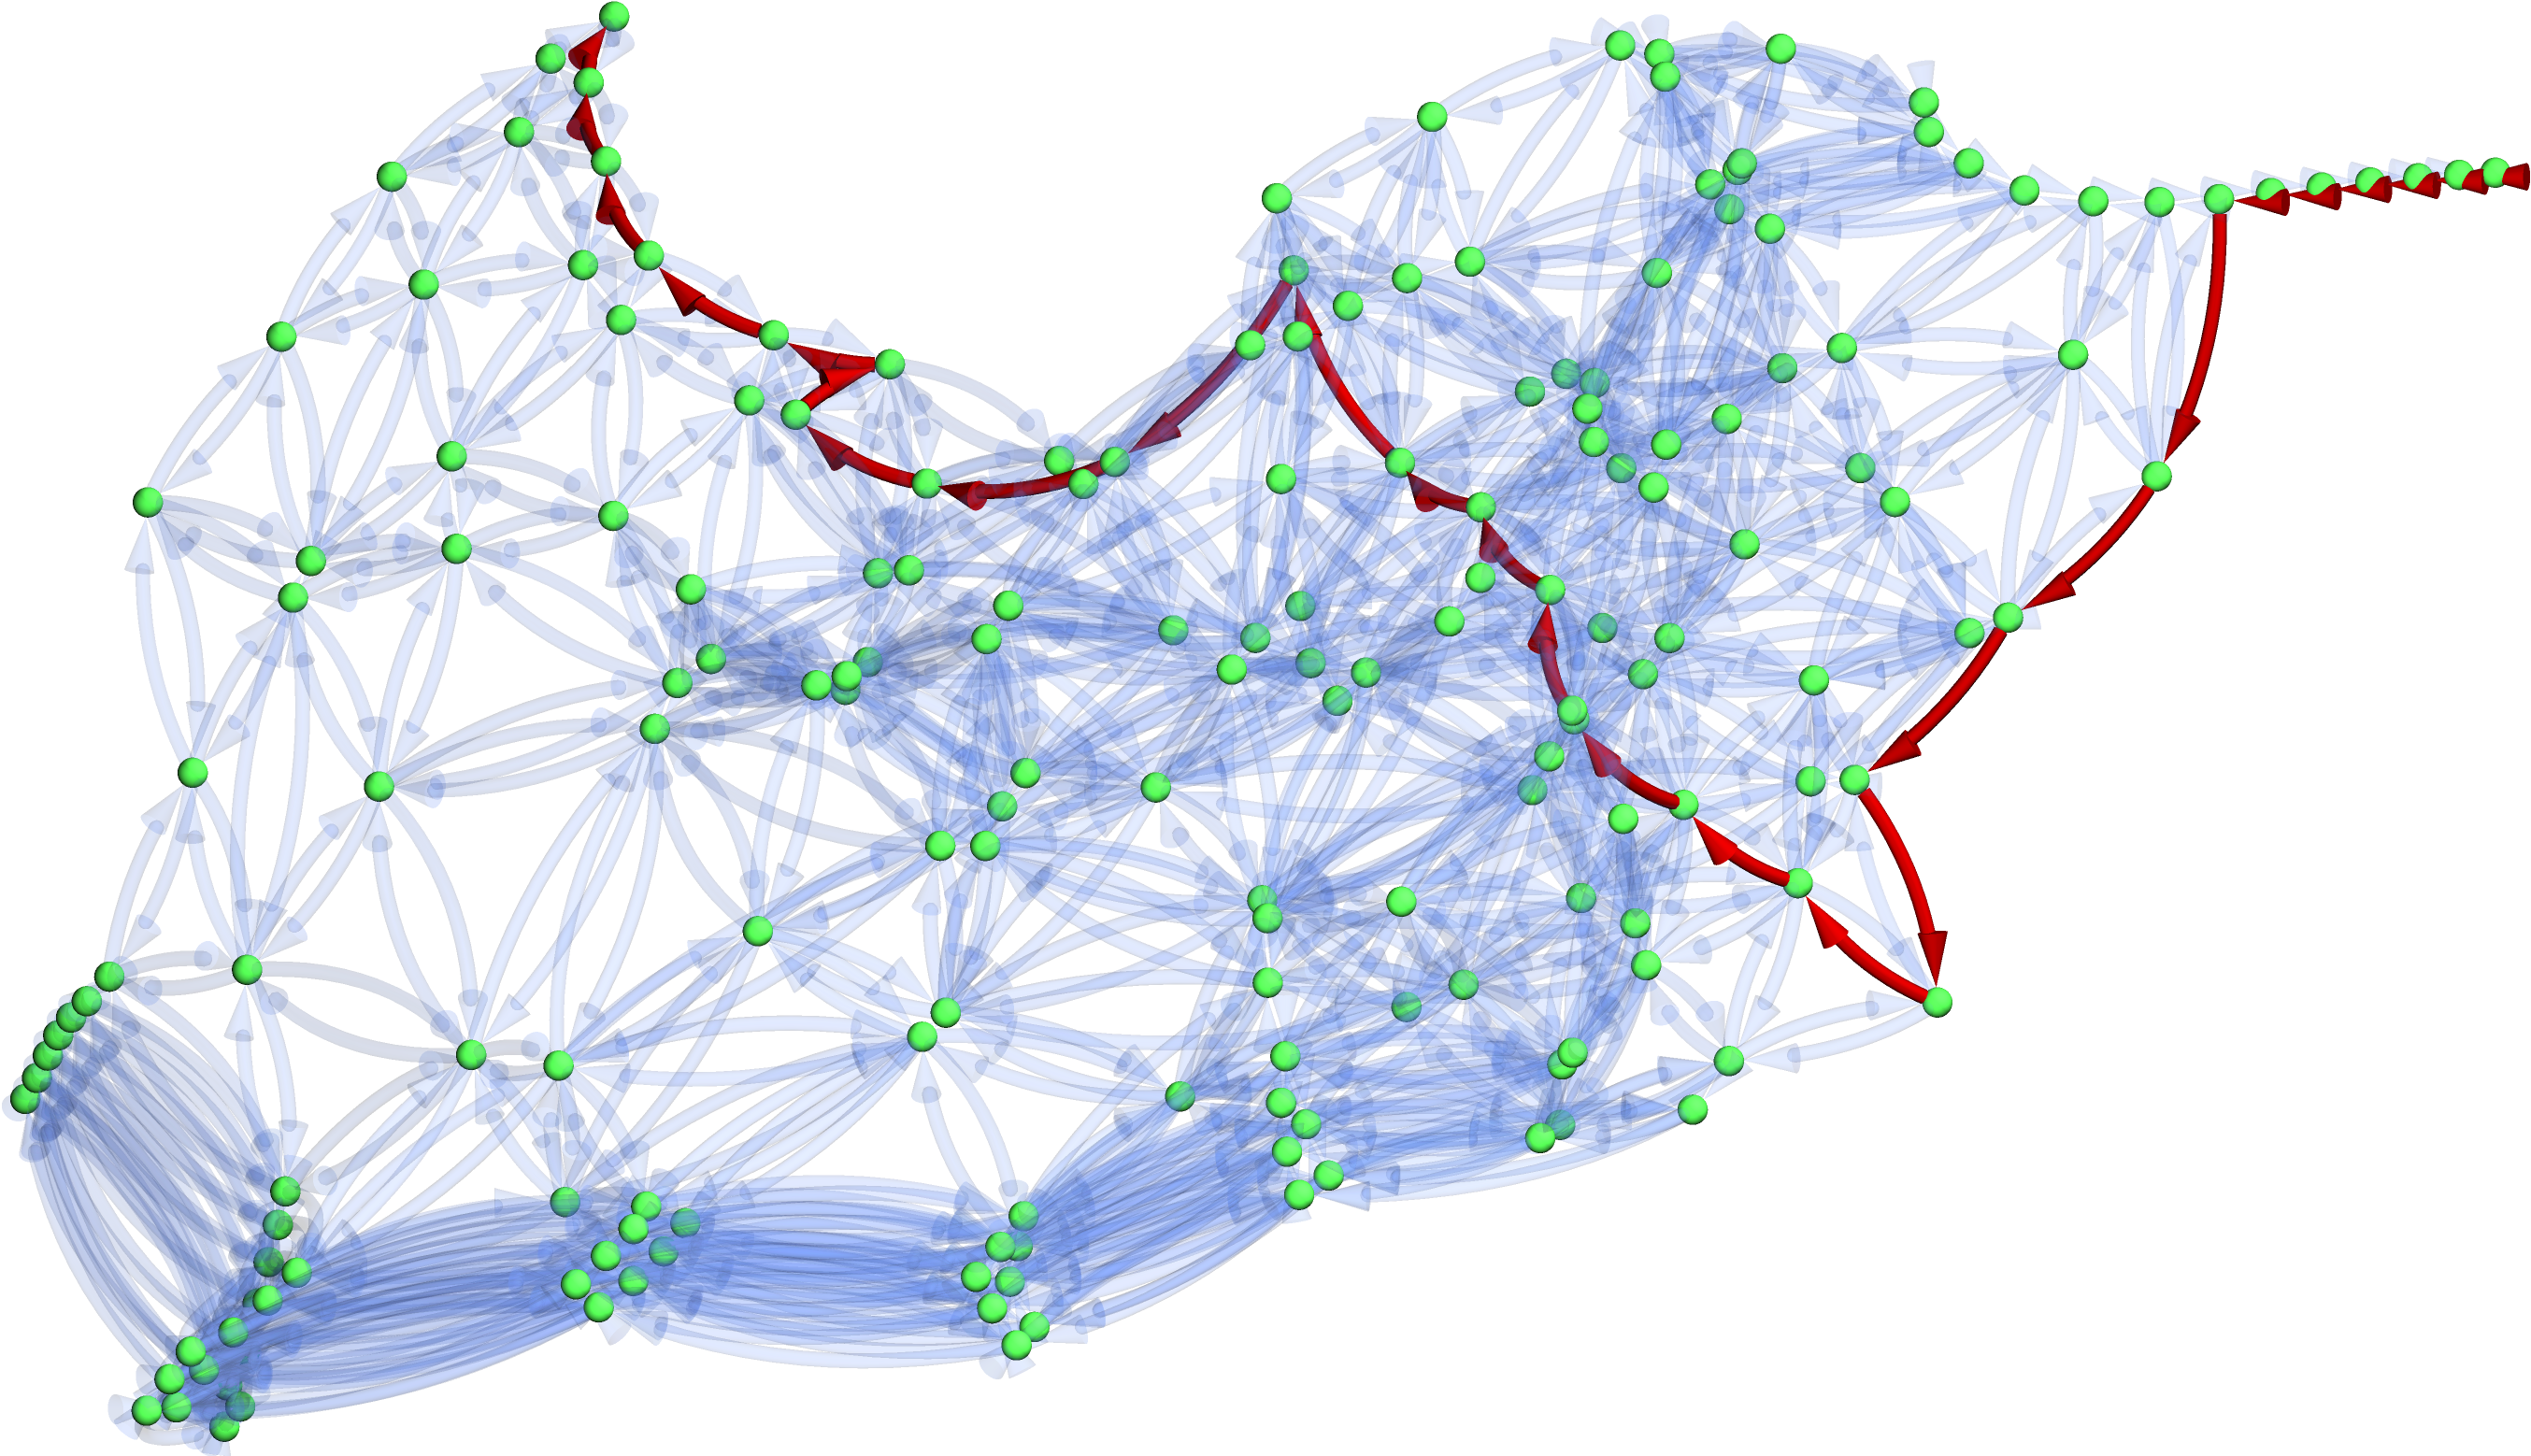
\includegraphics[width=0.9\textwidth]{pathplanning/InfeasibilityGliding_LowGradientSquared.png}
    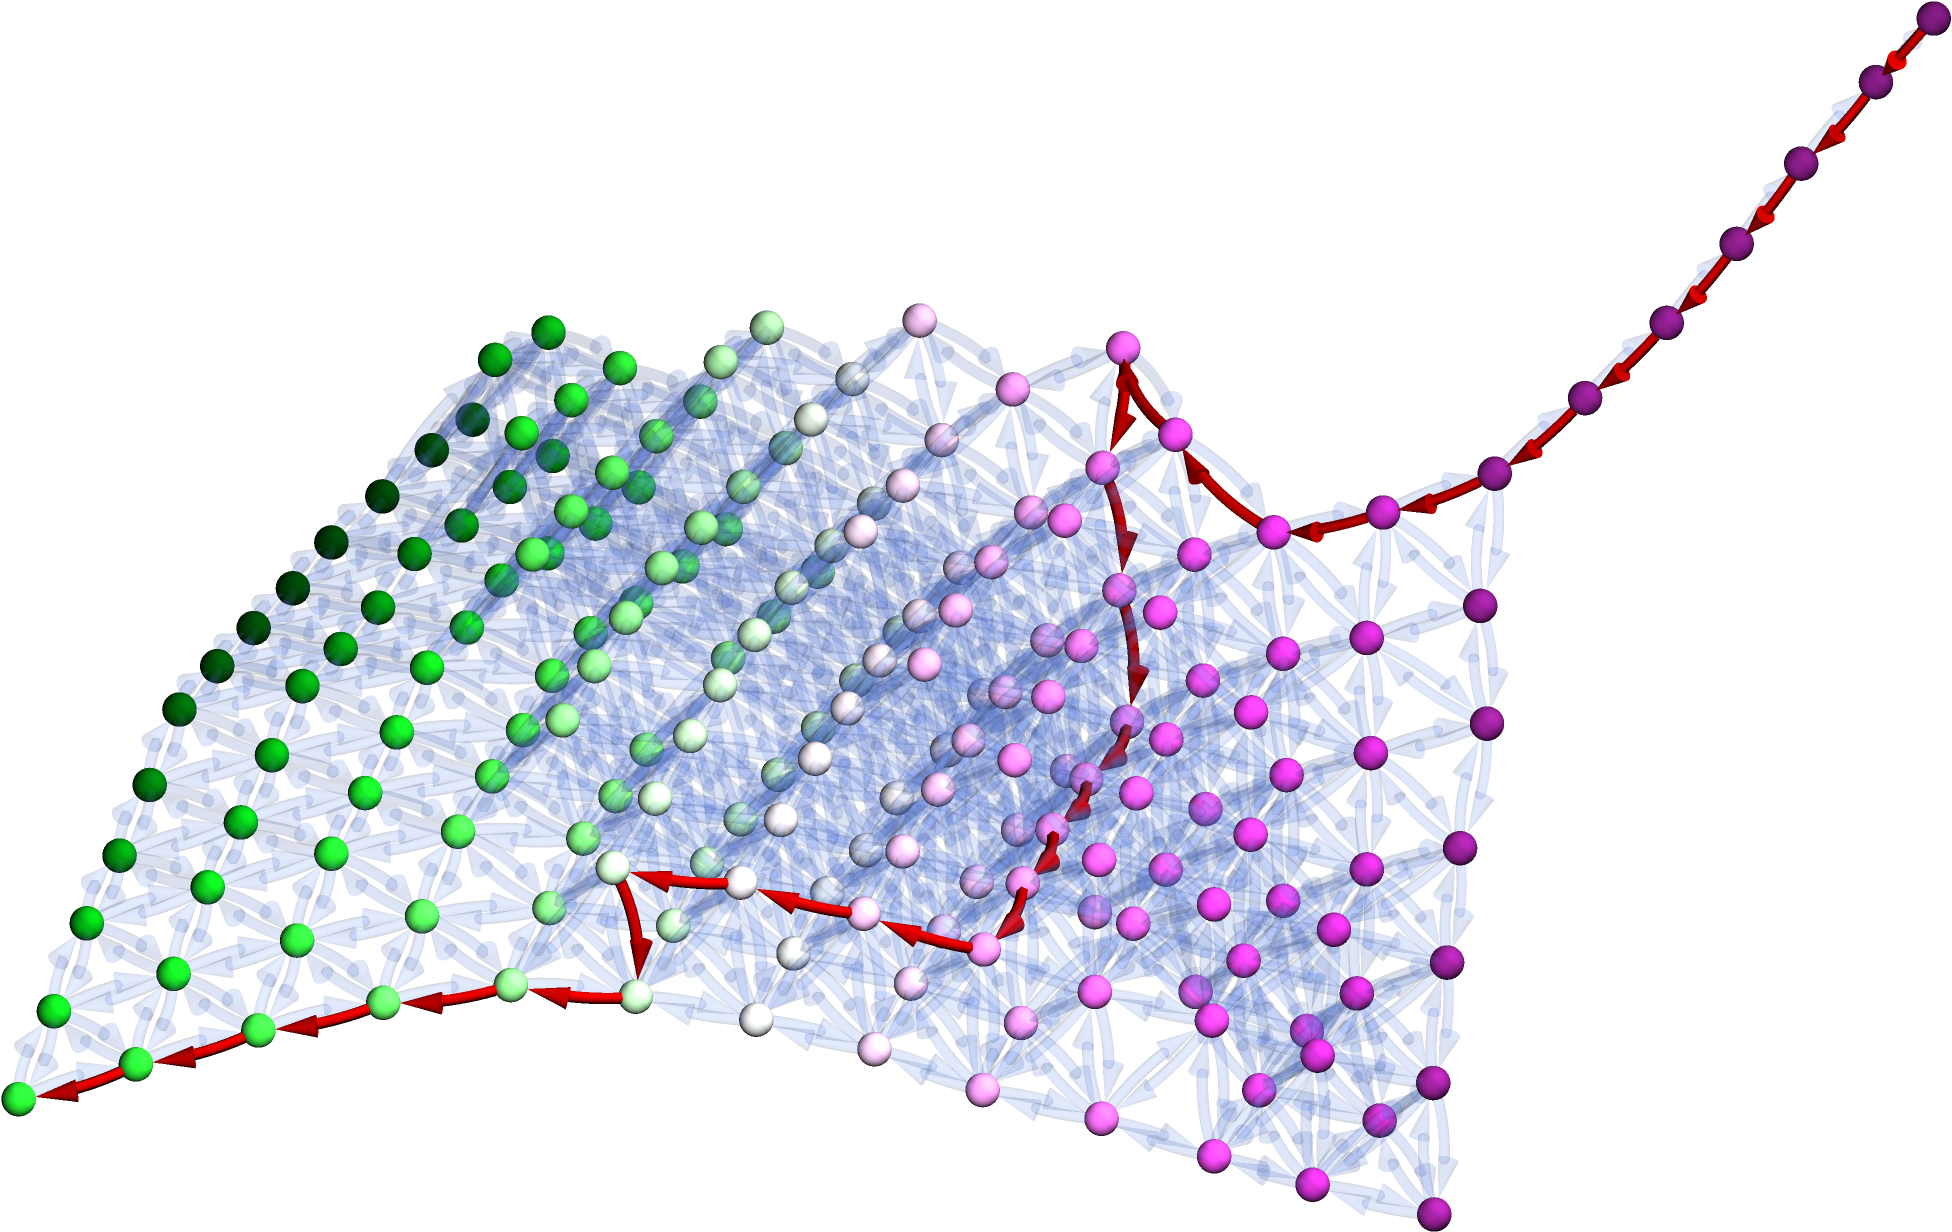
\includegraphics[width=0.9\textwidth]{pathplanning/InfeasibilityGliding_LowGradientSquaredColored.png}
    \caption{Application of a highly non-linear (squared) property gradient magnitude penalty to the inter-node distances causing (top) unrelaxable (local minimum) spatial arrangement of graph nodes, which can be visualized (bottom) through color encoding of property field with path forming "switchbacks" akin to mountain roads that minimize sharp gradients at a cost of 3 additional steps.}
    \label{pathplan:fig:lowgradientsquared}
\end{figure}

\section{Property Value Min/Maximization} \label{pathplan:sec:minmax}

\todo

Since the transitions between neighboring compositions are described through two unidirectional edges, the distance bias can be used to encode directional properties, such as the property gradient itself. Such method can be used to bias the path into crossing through high property value regions and, similar to those previously described, can be tuned to a desired trade-off with path length.

\begin{figure}[H]
    \centering
    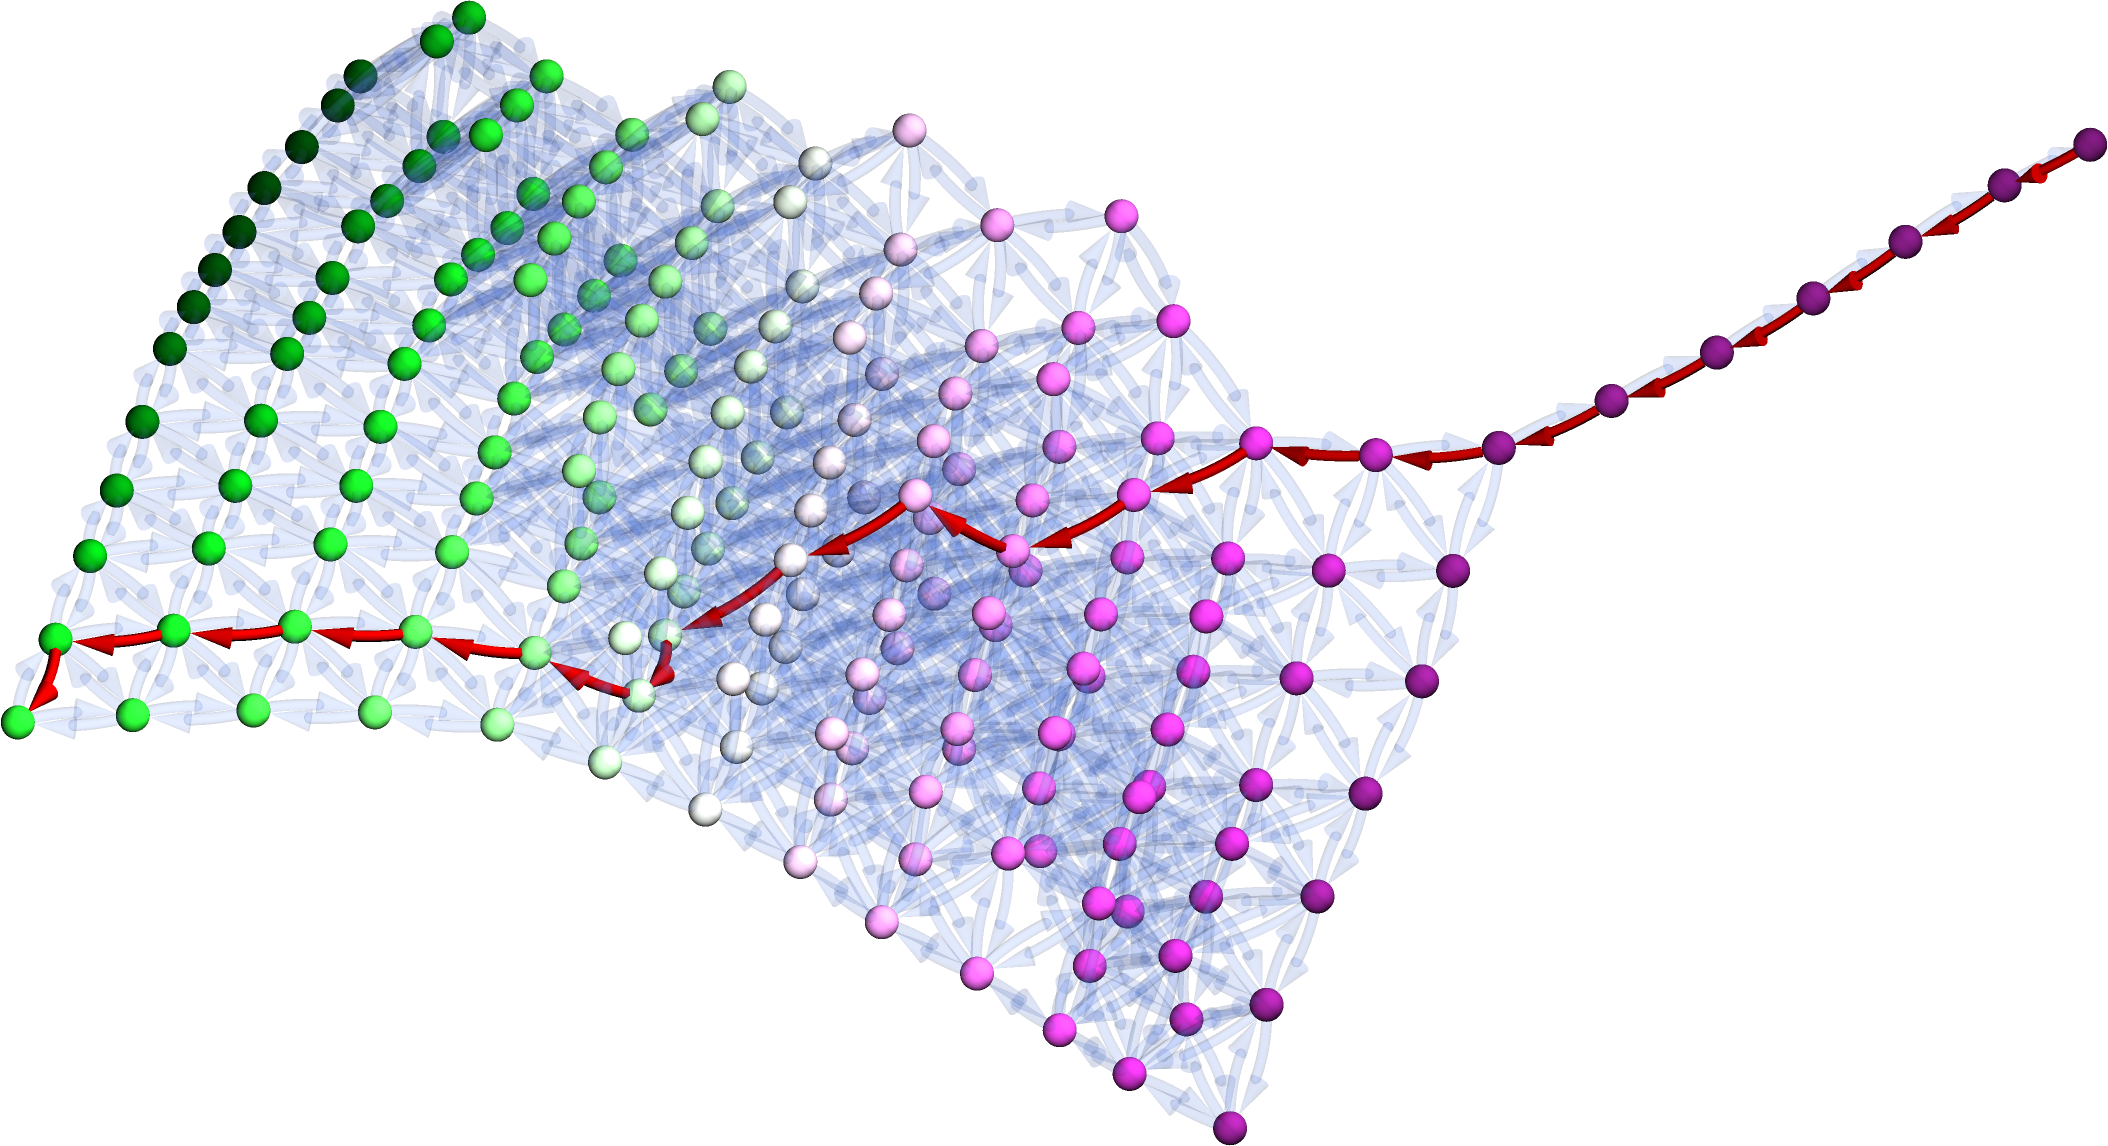
\includegraphics[width=0.9\textwidth]{pathplanning/InfeasibilityGliding_HighRMSAD.png}
    \caption{A selection of an optimal path, similar to one in Figure \ref{pathplan:fig:shortestpath} but biased towards high property value regions (green) by penalizing going to lower property regions.}
    \label{pathplan:fig:highrmsad}
\end{figure}


\printbibliography[heading=subbibintoc]